% patterns.meta family coverage: Lines, Hatch, Dots, Stars and options.
\usetikzlibrary{patterns.meta}

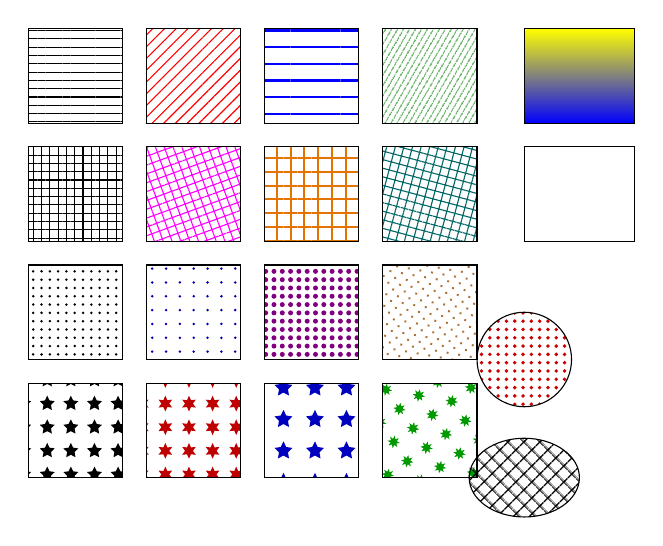
\begin{tikzpicture}[x=1cm,y=1cm,font=\scriptsize]
  % Lines family
  \path[draw,pattern={Lines},pattern color=black] (0,0) rectangle +(1.2,1.2);
  \path[draw,pattern={Lines[angle=45]},pattern color=red] (1.5,0) rectangle +(1.2,1.2);
  \path[draw,pattern={Lines[distance=6pt,line width=.8pt]},pattern color=blue] (3.0,0) rectangle +(1.2,1.2);
  \path[draw,pattern={Lines[distance={3pt/sqrt(2)},angle=60,xshift=1pt,yshift=2pt]},pattern color=green!50!black] (4.5,0) rectangle +(1.2,1.2);

  % Hatch family
  \path[draw,pattern={Hatch},pattern color=black] (0,-1.5) rectangle +(1.2,1.2);
  \path[draw,pattern={Hatch[angle=20]},pattern color=magenta] (1.5,-1.5) rectangle +(1.2,1.2);
  \path[draw,pattern={Hatch[distance=5pt,line width=.7pt]},pattern color=orange!90!black] (3.0,-1.5) rectangle +(1.2,1.2);
  \path[draw,pattern={Hatch[angle=75,xshift=1.5pt,yshift=-1pt]},pattern color=teal!80!black] (4.5,-1.5) rectangle +(1.2,1.2);

  % Dots family
  \path[draw,pattern={Dots},pattern color=black] (0,-3.0) rectangle +(1.2,1.2);
  \path[draw,pattern={Dots[distance=5pt]},pattern color=blue!70!black] (1.5,-3.0) rectangle +(1.2,1.2);
  \path[draw,pattern={Dots[radius=.9pt]},pattern color=violet] (3.0,-3.0) rectangle +(1.2,1.2);
  \path[draw,pattern={Dots[angle=35,xshift=1pt,yshift=1pt]},pattern color=brown!90!black] (4.5,-3.0) rectangle +(1.2,1.2);

  % Stars family
  \path[draw,pattern={Stars},pattern color=black] (0,-4.5) rectangle +(1.2,1.2);
  \path[draw,pattern={Stars[points=6]},pattern color=red!75!black] (1.5,-4.5) rectangle +(1.2,1.2);
  \path[draw,pattern={Stars[distance=4mm,radius=1.2mm]},pattern color=blue!75!black] (3.0,-4.5) rectangle +(1.2,1.2);
  \path[draw,pattern={Stars[angle=35,xshift=1pt,yshift=1pt,points=8,radius=.8mm]},pattern color=green!60!black] (4.5,-4.5) rectangle +(1.2,1.2);

  % Interaction checks
  \path[draw,pattern={Lines[angle=15]},pattern color=purple,top color=yellow,bottom color=blue] (6.3,0) rectangle +(1.4,1.2);
  \path[draw,fill=yellow!50,pattern=none] (6.3,-1.5) rectangle +(1.4,1.2);
  \path[draw,pattern={Dots[radius=.7pt]},pattern color=red!80!black] (6.3,-3.0) circle[radius=.6];
  \path[draw,pattern={Hatch[angle=45,distance=4pt,line width=.5pt]},pattern color=black] (6.3,-4.5) ellipse[x radius=.7,y radius=.5];
\end{tikzpicture}
